

\begin{frame}{Introdução}
  
Sistema que controla o tráfego de pacotes em uma rede de acordo com
regras pré-definidas.

\begin{figure}[ht]
\centering
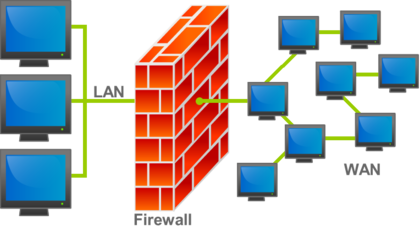
\includegraphics[scale=.7]{firewall.png}
\caption{Esquema de um firewall\footnote{\scriptsize Adaptado de
    \url{https://commons.wikimedia.org/wiki/File:Firewall.png}}.}
\end{figure}

\end{frame}

\begin{frame}{Ferramentas}

  Nos sistemas Linux o firewall normalmente utilizado é o
  \href{http://www.netfilter.org/projects/iptables/}{iptables}, e nos
  sistemas BSD, o \href{http://www.openbsd.org/faq/pf/}{pf} ({\em packet
    filter}).

\end{frame}

\begin{frame}{Regras de bloqueio}

  O firewall utiliza algumas características dos pacotes na rede,
  dentre elas:

\begin{itemize}
\item Porta de origem;
\item IP de destino;
\item Porta de destino;
\item Protocolo IP (TCP ou UDP).
\end{itemize}

\end{frame}
